\chapter{Self-organized criticality and sandpile models}
\label{ch:soc}

\newcommand{\socHeightSim}[1]{\ifcase#1 0.0738\or 0.1739\or 0.3057\or 0.4465\fi}
\newcommand{\socMeanHeightSim}{2.1249}
\newcommand{\socLmax}{512}
\newcommand{\socNav}{1{,}000{,}000}
\newcommand{\socDest}{2.81}
\newcommand{\socTauRel}{1.29}
\newcommand{\socMeanSim}{9299}
\newcommand{\socMeanExact}{9285}


This chapter develops the ideas needed to talk precisely about ``criticality'' in an
earthquake model. \Cref{sec:pl} defines probability distributions and power laws and
explains what makes power laws special. \Cref{sec:critical} recalls where power laws
appear in ordinary statistical physics, at critical points, using percolation as the
example. \Cref{sec:soc} presents the idea of self-organized criticality. The rest of the
chapter studies the Bak--Tang--Wiesenfeld (BTW) sandpile: its definition
(\cref{sec:btw-def}), its remarkable Abelian property (\cref{sec:abelian}), its long-time
behaviour (\cref{sec:stationary}), an exact formula for the mean avalanche size
(\cref{sec:mean}), a complete solution in one dimension (\cref{sec:btw1d}), and its
behaviour in two dimensions (\cref{sec:btw2d}). The chapter closes with what these results
imply for the Burridge--Knopoff model (\cref{sec:soc-implications}).

% ======================================================================
\section{Probability distributions and power laws}
\label{sec:pl}

\subsection{Basic definitions}

Throughout this thesis we deal with quantities that vary randomly from one event to the next:
the size of an avalanche, the moment of an earthquake. Let $x$ be such a quantity.

\begin{definition}
The \emph{probability density} $P(x)$ is defined so that $P(x)\,\dd x$ is the probability that
the quantity lies between $x$ and $x+\dd x$. It is non-negative and normalised,
$\int P(x)\,\dd x = 1$. If $x$ takes only integer values, as the number of topplings in an
avalanche does, $P(x)$ is the probability of the value $x$ and integrals become sums; we use the
same notation for both cases.
\end{definition}

\begin{definition}
The \emph{complementary cumulative distribution} is the probability that the quantity is at
least $x$,
\begin{equation}
  \bar F(x) = \int_x^\infty P(x')\,\dd x' , \qquad\text{so that}\qquad P(x) = -\frac{\dd \bar F}{\dd x}.
  \label{eq:Fbar}
\end{equation}
\end{definition}
The Gutenberg--Richter count $N(\geq M_w)$ of Chapter~\ref{ch:intro} is, up to the total number of
events, a complementary cumulative distribution.

\begin{definition}
The \emph{$q$-th moment} of the distribution is the average of $x^q$,
\begin{equation}
  \avg{x^q} = \int x^q P(x)\,\dd x .
\end{equation}
The first moment $\avg{x}$ is the mean.
\end{definition}

\subsection{Power laws}

\begin{definition}
A distribution is a \emph{power law} with \emph{exponent} $\tau$ if
\begin{equation}
  P(x) = C\, x^{-\tau}\qquad\text{for } x \ge x_{\min},
  \label{eq:pl}
\end{equation}
where $C$ is a normalisation constant and $x_{\min}>0$ is the smallest value considered.
\end{definition}

\paragraph{Why logarithmic axes.} Taking the logarithm of \cref{eq:pl} gives
\begin{equation}
  \log P = \log C - \tau \log x .
\end{equation}
In a plot of $\log P$ against $\log x$ (a ``log--log plot'') a power law is therefore a straight
line with slope $-\tau$. This is why distributions of avalanche and earthquake sizes are almost
always shown on logarithmic axes.

\paragraph{Normalisation.} The lower limit $x_{\min}$ is necessary: the integral of $x^{-\tau}$
diverges at $x\to0$ for every $\tau\ge1$. With $x_{\min}$ in place,
\begin{equation}
  \int_{x_{\min}}^{\infty} C x^{-\tau}\,\dd x
  = C \left[\frac{x^{1-\tau}}{1-\tau}\right]_{x_{\min}}^{\infty}
  = C\,\frac{x_{\min}^{1-\tau}}{\tau-1}\qquad(\tau>1).
\end{equation}
Setting this equal to 1 gives $C = (\tau-1)\,x_{\min}^{\tau-1}$. For $\tau\le1$ the integral diverges
at large $x$ and the distribution cannot be normalised without an upper limit as well.

\paragraph{Cumulative distribution.} Using \cref{eq:Fbar},
\begin{equation}
  \bar F(x) = \int_x^\infty (\tau-1)x_{\min}^{\tau-1}\, x'^{-\tau}\,\dd x'
  = \left(\frac{x}{x_{\min}}\right)^{-(\tau-1)} .
  \label{eq:Fbar-pl}
\end{equation}
The cumulative distribution of a power law is again a power law, with exponent smaller by one. This is
exactly the relation between the exponent $2b/3$ of the cumulative Gutenberg--Richter law and the
exponent $\tau = 1 + 2b/3$ of the density, found in \cref{eq:GR-density}.

\paragraph{The mean.} The mean of a pure power law is
\begin{equation}
  \avg{x} = \int_{x_{\min}}^{\infty} x\cdot C x^{-\tau}\,\dd x = C\left[\frac{x^{2-\tau}}{2-\tau}\right]_{x_{\min}}^{\infty}
  = \frac{\tau-1}{\tau-2}\,x_{\min}\qquad(\tau>2),
\end{equation}
and it is infinite for $\tau\le 2$. For the exponents met in this thesis ($1<\tau\le2$) the mean of a real,
finite system is therefore controlled by its \emph{largest} values. If the power law holds up to an upper
cutoff $x_c\gg x_{\min}$,
\begin{equation}
  \avg{x} \approx C\int_{x_{\min}}^{x_c} x^{1-\tau}\,\dd x = C\,\frac{x_c^{2-\tau} - x_{\min}^{2-\tau}}{2-\tau}
  \approx \frac{C}{2-\tau}\, x_c^{\,2-\tau}\qquad(1<\tau<2).
  \label{eq:mean-cutoff}
\end{equation}
The mean grows without bound as the cutoff grows. This simple formula will give an exact relation between
exponents in \cref{sec:mean}.

\subsection{Scale invariance}
\label{sec:scaleinv}

What makes power laws special is that they have \emph{no characteristic scale}. To see what this means,
compare a power law with an exponential distribution, $P(x)\propto e^{-x/\xi}$. The exponential contains a
scale $\xi$: values of $x$ much smaller than $\xi$ are common, values much larger than $\xi$ are
astronomically rare. If someone shows you a plot of the exponential over a window $[x_0, 10x_0]$, you can tell
from the shape where you are: for $x_0\ll\xi$ the curve is almost flat, for $x_0\gg\xi$ it drops like a cliff.

A power law looks the same in every window. Change the unit in which $x$ is measured by a factor $\lambda$:
\begin{equation}
  P(\lambda x) = C\,(\lambda x)^{-\tau} = \lambda^{-\tau}\,P(x).
  \label{eq:scaleinv}
\end{equation}
The rescaled function is the old function multiplied by a constant. On a plot where the vertical axis is
normalised to the value at the start of the window, all windows give the same curve
(\cref{fig:scaleinv}).

\begin{figure}[t]
  \centering
  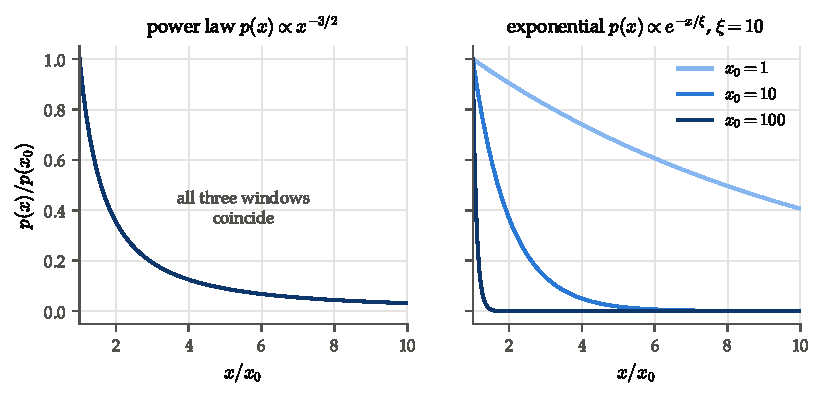
\includegraphics[width=\linewidth]{soc/scale_invariance.pdf}
  \caption{The same distribution seen through three windows $[x_0, 10x_0]$, with $x_0=1,10,100$. Each curve
  is divided by its value at the start of the window. Left: a power law gives the same curve in every window.
  Right: an exponential with scale $\xi=10$ looks completely different in each window.}
  \label{fig:scaleinv}
\end{figure}

Remarkably, the converse is also true: \emph{the power law is the only scale-invariant function}. Suppose
that rescaling $x$ by any factor $\lambda$ only multiplies $P$ by a factor $f(\lambda)$ that does not
depend on $x$:
\begin{equation}
  P(\lambda x) = f(\lambda)\,P(x)\qquad\text{for all } x,\lambda>0 .
  \label{eq:scaleinv-general}
\end{equation}
\begin{enumerate}
  \item Rescaling first by $\lambda_2$ and then by $\lambda_1$ is the same as rescaling once by
    $\lambda_1\lambda_2$. Applying \cref{eq:scaleinv-general} twice,
    $P(\lambda_1\lambda_2 x) = f(\lambda_1)f(\lambda_2)P(x)$; applying it once,
    $P(\lambda_1\lambda_2x) = f(\lambda_1\lambda_2)P(x)$. Hence
    \begin{equation}
      f(\lambda_1\lambda_2) = f(\lambda_1)\,f(\lambda_2).
    \end{equation}
  \item Differentiate with respect to $\lambda_1$ and then set $\lambda_1=1$:
    $\lambda_2 f'(\lambda_2) = f'(1)\,f(\lambda_2)$. Call the constant $f'(1) = -\tau$.
  \item The equation $\lambda f'(\lambda) = -\tau f(\lambda)$ is separable:
    $\dd f/f = -\tau\,\dd\lambda/\lambda$, so $\ln f = -\tau\ln\lambda + \text{const}$. Since $f(1)=1$,
    the constant is zero and $f(\lambda) = \lambda^{-\tau}$.
  \item Finally put $x=1$ in \cref{eq:scaleinv-general}: $P(\lambda) = \lambda^{-\tau}P(1)$. Renaming
    $\lambda\to x$, $P(x) = P(1)\,x^{-\tau}$, a power law.
\end{enumerate}

So when we observe a power law over many decades, we are observing a system in which nothing selects a
particular size. In physics, the classic situation where this happens is a critical point.

\paragraph{Cutoffs.} No real distribution is a power law for all $x$. There is always a smallest unit (one
grain, one block) and a largest possible event (set by the size of the system). A realistic form is
\begin{equation}
  P(x) = x^{-\tau}\,\mathcal{G}\!\left(\frac{x}{x_c}\right),
  \label{eq:cutoff-form}
\end{equation}
where the \emph{cutoff function} $\mathcal G(u)$ is approximately constant for $u\ll1$ and decays rapidly
for $u\gg1$, and $x_c$ is the \emph{cutoff}. The power law then holds in the window $x_{\min}\ll x\ll x_c$.
The important questions are what the exponent $\tau$ is in that window and how $x_c$ depends on the size of
the system.

% ======================================================================
\section{Power laws at critical points}
\label{sec:critical}

\subsection{Phase transitions}

A \emph{phase transition} is a qualitative change in the large-scale state of a system when a
\emph{control parameter} is varied: water boils when the temperature passes \SI{100}{\celsius} at
atmospheric pressure, and a piece of iron loses its magnetisation when heated above its Curie temperature,
about \SI{770}{\celsius}. The state on each side of the transition is characterised by an \emph{order
parameter}, a quantity that is zero in one phase and non-zero in the other, such as the magnetisation of the
iron.

Transitions come in two kinds. At a \emph{first-order} transition the order parameter jumps (liquid water
and steam have different densities at the boiling point). At a \emph{continuous} or \emph{critical}
transition it goes to zero continuously, and something remarkable happens: the system develops fluctuations
on all length scales at once. A fluid near its critical point becomes milky (``critical opalescence''),
because density fluctuations of all sizes, including sizes comparable to the wavelength of light, are present.

The quantity that makes this precise is the \emph{correlation length} $\xi$. It is the distance over which
the state of one part of the system influences the state of another part: two points much closer than $\xi$
behave in a correlated way, two points much farther apart than $\xi$ behave independently. Away from the
critical point $\xi$ is finite, a few molecular distances. At the critical point it diverges. Near the
critical point it diverges as a power of the distance from it, for example
\begin{equation}
  \xi \propto |T - T_c|^{-\nu},
\end{equation}
where $T_c$ is the critical temperature and $\nu$ is a \emph{critical exponent}. Other quantities have their
own exponents. A key discovery of the theory of critical phenomena is \emph{universality}: the critical
exponents do not depend on the details of a system, only on a few general properties such as the dimension
of space and the symmetries. The liquid--gas critical point of carbon dioxide and the critical point of a
certain class of magnets have the same exponents. This is why very simple models can predict exponents of
real systems exactly.

\subsection{Percolation: a geometric critical point}

The simplest model with a critical point is \emph{percolation}~\cite{Stauffer1994}. Each site of a lattice
is occupied with probability $p$ and empty with probability $1-p$, independently of all other sites.
Neighbouring occupied sites form \emph{clusters} (\cref{fig:percolation}). The control parameter is $p$.

\begin{figure}[t]
  \centering
  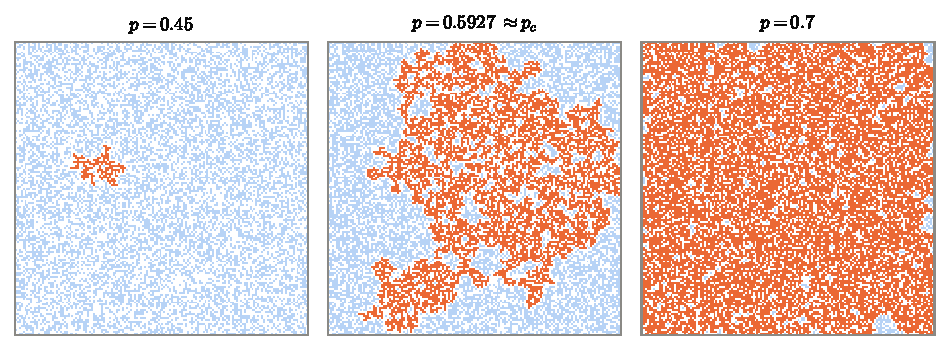
\includegraphics[width=\linewidth]{soc/percolation.pdf}
  \caption{Site percolation on a $150\times150$ square lattice. Occupied sites are light blue, and the largest
  cluster is orange. Below the threshold (left) the largest cluster is small. At the threshold
  $p_c\approx0.5927$ (middle) it is a ragged, fractal object with holes of all sizes. Above it (right) it fills
  most of the lattice.}
  \label{fig:percolation}
\end{figure}

For small $p$ the clusters are small and isolated. For $p$ close to 1 almost everything is connected into one
huge cluster. In between, at a sharp \emph{percolation threshold} $p_c$ ($p_c\approx 0.5927$ for sites of the
square lattice), an infinite cluster appears for the first time. The order parameter is the probability that a
site belongs to the infinite cluster. The correlation length is the typical radius of the finite clusters, and
it diverges at the threshold, $\xi\propto|p-p_c|^{-\nu}$ with $\nu = 4/3$ in two dimensions.

The cluster sizes are described by the \emph{cluster number} $n_s$, the number of clusters containing exactly
$s$ sites, divided by the number of lattice sites. Near $p_c$ it has the form
\begin{equation}
  n_s \simeq s^{-\tau}\,\mathcal G\!\left(\frac{s}{s_\xi}\right),\qquad s_\xi \propto \xi^{D},
  \label{eq:perc-scaling}
\end{equation}
which is exactly the cutoff form \cref{eq:cutoff-form}. In two dimensions $\tau = 187/91\approx2.06$. The
cutoff $s_\xi$ is the size of a cluster whose radius is $\xi$, and $D=91/48\approx1.90$ is the \emph{fractal
dimension} of the clusters: a cluster of radius $R$ contains about $R^{D}$ sites, fewer than the $R^2$ sites of
a filled disc, because it is full of holes (\cref{fig:percolation}, middle). Only exactly at $p=p_c$, where
$s_\xi=\infty$, is the cluster distribution a pure power law.

\subsection{One-dimensional percolation, worked out}
\label{sec:perc1d}

In one dimension percolation can be solved with elementary probability, and the solution is instructive
because the same features will appear in the one-dimensional sandpile.

\paragraph{Cluster numbers.} On a chain, a cluster of exactly $s$ sites that starts at a given site $i$ requires
sites $i,\dots,i+s-1$ to be occupied (probability $p^s$) and the two sites just outside, $i-1$ and $i+s$, to be
empty (probability $(1-p)^2$). Hence
\begin{equation}
  n_s = (1-p)^2\, p^{s} = (1-p)^2\, e^{-s/s_\xi},\qquad s_\xi = -\frac{1}{\ln p} .
\end{equation}
This is an \emph{exponential}, not a power law: for every $p<1$ there is a characteristic cluster size $s_\xi$.

\paragraph{Mean cluster size.} Pick an occupied site at random and ask for the size of its cluster. A cluster of
size $s$ contains $s$ sites, so the probability that the chosen site belongs to a cluster of size $s$ is
proportional to $s\,n_s$. The mean cluster size is therefore $S = \sum_s s^2 n_s / \sum_s s\,n_s$. Using the sums
$\sum_{s\ge1} s\,p^s = p/(1-p)^2$ and $\sum_{s\ge1}s^2p^s = p(1+p)/(1-p)^3$,
\begin{equation}
  \sum_s s\, n_s = (1-p)^2\frac{p}{(1-p)^2} = p, \qquad
  \sum_s s^2 n_s = (1-p)^2\frac{p(1+p)}{(1-p)^3} = \frac{p(1+p)}{1-p},
\end{equation}
\begin{equation}
  S = \frac{1+p}{1-p} .
\end{equation}
(The first sum is a check: it is the fraction of occupied sites, $p$.) The mean cluster size diverges as
$(1-p)^{-1}$ when $p\to1$, a power law with exponent $\gamma=1$.

\paragraph{Correlation length.} Two sites at distance $r$ belong to the same cluster only if all $r+1$ sites from
one to the other are occupied. Given that the first is occupied, this has probability $p^{r} = e^{-r/\xi}$ with
$\xi = -1/\ln p$. As $p\to1$, $\ln p\approx -(1-p)$ and $\xi\approx(1-p)^{-1}$, so $\nu = 1$.

\paragraph{Lesson.} The critical point of one-dimensional percolation is at $p_c = 1$, the very edge of the range
of $p$. There the ``critical state'' is the trivial fully occupied chain, with a single cluster. A single empty
site cuts a chain, so in one dimension it is very hard to build long-range connections. One-dimensional
systems are special in this way, and we will meet the same situation in the sandpile.

\subsection{The problem of fine tuning}

In all these examples a power law appears only at one special value of the control parameter ($T_c$, $p_c$).
An experimentalist who wants to observe it must tune the parameter to that value with great precision. But
earthquakes obey the Gutenberg--Richter law everywhere, and nobody tunes the Earth's crust. This puzzle is
the starting point of self-organized criticality.

% ======================================================================
\section{Self-organized criticality}
\label{sec:soc}

\subsection{The idea}

In 1987 Bak, Tang and Wiesenfeld~\cite{BTW1987,BTW1988} proposed that some systems are driven \emph{to} a
critical point by their own dynamics. They called this \emph{self-organized criticality} (SOC). In the
self-organized critical state a small perturbation can trigger a response, an \emph{avalanche}, of any size, and
the sizes follow a power law, without any parameter having been tuned. The systems they had in mind share four
ingredients~\cite{Jensen1998,Charbonneau2017}:
\begin{enumerate}
  \item \textbf{Slow driving.} Some quantity (sand, stress, energy) is added to the system slowly, a little at a
    time.
  \item \textbf{A local threshold.} Nothing happens at a point of the system until a local variable exceeds a
    critical value. Below the threshold the system is stable; it can store the added quantity.
  \item \textbf{Fast local relaxation.} When the threshold is exceeded at a point, the quantity stored there is
    passed to the neighbouring points. They may exceed their own threshold and pass it on, and so on: this
    chain reaction is the avalanche.
  \item \textbf{Dissipation.} The quantity must be able to leave the system, for example through its boundary;
    otherwise it would accumulate forever and no steady state could exist.
\end{enumerate}
The driving must be slow compared with the relaxation: an avalanche must be finished before the next unit is
added, so that avalanches are distinct events. This is the \emph{separation of time scales}.

\Cref{tab:soc-analogy} shows how these ingredients appear in a sandpile and in an earthquake fault. The
separation of time scales on a real fault, estimated in \cref{sec:stickslip}, is about $10^{-8}$.

\begin{table}[t]
\centering
\caption{The ingredients of self-organized criticality in a sandpile and in an earthquake fault.}
\label{tab:soc-analogy}
\begin{tabular}{@{}p{22mm}p{50mm}p{70mm}@{}}
\toprule
ingredient & sandpile & earthquake fault (BK model) \\
\midrule
slow drive & grains added one at a time & plate moves at velocity $v$ \\
threshold & critical height $z_c$ & maximum static friction $F_0$ \\
relaxation & toppling to neighbours & slip; force passed through coupling springs $k_c$ \\
dissipation & grains leave at the boundary & energy lost to friction; stress taken up by pulling springs $k_p$ \\
\bottomrule
\end{tabular}
\end{table}

\subsection{Why the critical point is an attractor}

The reason a system can organise itself to a critical point can be understood with a feedback argument.
Think of a sandpile with some average density of grains $\zeta$. If the density is low, an added grain causes
only a small avalanche, which does not reach the boundary: grains accumulate and $\zeta$ increases. If the
density is high, added grains cause huge avalanches that carry many grains out through the boundary: $\zeta$
decreases. The density is pushed towards the special value $\zeta_c$ between the two regimes, where avalanches
are just barely able to propagate to any distance. That value is a critical point, and the slow drive and the
boundary dissipation together hold the system there.

This argument also shows the limits of the idea. The critical density is reached only if the drive is slow
enough (otherwise avalanches overlap and the system is pushed above $\zeta_c$) and if grains are lost only at the
boundary (if grains are lost inside the system, avalanches die out before they reach a large size, and the
system settles below $\zeta_c$). In a precise sense, then, ``self-organized'' criticality still needs two
parameters to be at a limiting value: the driving rate and the bulk dissipation must both go to zero. This view,
that SOC is an ordinary critical point whose control parameter is tuned automatically by a feedback, was made
precise by Dickman, Vespignani and Zapperi~\cite{DickmanVespignaniZapperi1998}. It is directly relevant to
earthquake models, in which the pulling springs remove stress inside the system: we will see in Chapter~4 that
Carlson and collaborators found the size of the largest ``critical'' events of the Burridge--Knopoff model to be
controlled by exactly such parameters.

% ======================================================================
\section{The Bak--Tang--Wiesenfeld sandpile}
\label{sec:btw-def}

\subsection{Definition}

The BTW sandpile is defined on a lattice: a chain of $L$ sites in one dimension, or a square grid of $L\times L$
sites in two dimensions. The sites are numbered $i=1,\dots,N$, with $N=L$ or $N = L^2$. Each site has a set of
\emph{neighbours}: on the chain, the sites to its left and right; on the square lattice, the four sites above,
below, left and right. The number of neighbours of a site in the interior is called $k$ ($k=2$ in one dimension,
$k=4$ in two). Sites on the edge of the lattice have fewer neighbours inside the lattice; we say that their
missing neighbours are ``outside''.

The state of the system is described by integers $z_i\ge0$, called \emph{heights}, which we picture as the
number of grains of sand at each site. The dynamics has two parts.
\begin{enumerate}
  \item \textbf{Driving.} Choose a site $j$ at random, each site with equal probability $1/N$, and add one grain:
    $z_j\to z_j+1$.
  \item \textbf{Toppling.} A site is \emph{stable} if $z_i < z_c$ and \emph{unstable} if $z_i\ge z_c$, where
    $z_c = k$ is the \emph{critical height}. An unstable site \emph{topples}: it loses $k$ grains, and each of its
    $k$ neighbours gains one grain,
    \begin{equation}
      z_i \to z_i - k,\qquad z_{m} \to z_{m}+1 \ \text{ for every neighbour } m \text{ of } i.
    \end{equation}
    If $i$ is on the edge, the grains sent to its missing neighbours fall off the lattice and are lost.
\end{enumerate}
After a grain is added, topplings continue until all sites are stable again. The sequence of topplings caused by
one added grain is an \emph{avalanche}. Only when the avalanche is over is the next grain added: this is the
separation of time scales of \cref{sec:soc}, built into the rules. Grains are conserved in every toppling except
those of edge sites, so the edges play the role of dissipation. A lattice whose edges lose grains in this way is
said to have \emph{open boundaries}.

The possible heights of a stable site are $0,1,\dots,k-1$: $0$ or $1$ on the chain, and $0,1,2,3$ on the square
lattice. The toppling rule is illustrated in \cref{fig:toppling}.

\begin{figure}[t]
\centering
\begin{tikzpicture}[x=9mm,y=9mm,>={Stealth[length=1.6mm]}]
  \foreach \i/\h in {1/1,2/1,3/2,4/0,5/1} {
    \draw[ink2,fill=\ifnum\h>1 corange!25\else cblue!10\fi] (\i-0.4,0) rectangle (\i+0.4,0.7);
    \node[font=\small] at (\i,0.35) {\h};
  }
  \node[font=\small,ink2] at (-0.1,0.35) {outside};
  \node[font=\small,ink2] at (6.1,0.35) {outside};
  \draw[->,corange,thick] (3,0.85) to[bend right=40] (2,0.85);
  \draw[->,corange,thick] (3,0.85) to[bend left=40] (4,0.85);
  \node[font=\footnotesize,ink2,align=center] at (3,-0.6) {chain, $k=2$: site 3 is unstable;\\it loses 2 grains, sites 2 and 4 gain 1 each};
  \begin{scope}[xshift=72mm,yshift=-4mm]
  \foreach \x in {0,1,2} \foreach \y in {0,1,2} {
    \pgfmathtruncatemacro\c{(\x==1 && \y==1)}
    \ifnum\c=1 \def\fillc{corange!25}\else\def\fillc{cblue!10}\fi
    \draw[ink2,fill=\fillc] (\x-0.4,\y-0.4) rectangle (\x+0.4,\y+0.4);
  }
  \node[font=\small] at (1,1) {4};
  \foreach \dx/\dy in {1/0,-1/0,0/1,0/-1} \draw[->,corange,thick] (1+0.25*\dx,1+0.25*\dy) -- (1+0.75*\dx,1+0.75*\dy);
  \node[font=\footnotesize,ink2,align=center] at (1,-1.1) {square lattice, $k=4$:\\one grain to each neighbour};
  \end{scope}
\end{tikzpicture}
\caption{The toppling rule of the BTW sandpile.}
\label{fig:toppling}
\end{figure}

\subsection{Measuring an avalanche}

For each added grain we record four numbers:
\begin{itemize}[nosep]
  \item the \textbf{size} $s$: the total number of topplings;
  \item the \textbf{area} $a$: the number of different sites that toppled at least once;
  \item the \textbf{duration} $T$: the number of time steps, where in each time step all the sites that are
    unstable at the beginning of the step topple once, simultaneously (the \emph{parallel update});
  \item the number of grains \textbf{lost} through the boundary.
\end{itemize}

\begin{example}
\label{ex:avalanche}
Take a chain of $L=5$ sites with heights $(1,1,1,1,0)$ and add a grain at site $j=2$. The avalanche proceeds as
follows (unstable sites in bold):
\begin{center}
\begin{tabular}{clc}
\toprule
step & heights & sites that topple \\
\midrule
start & $(1,\mathbf{2},1,1,0)$ & 2 \\
1 & $(\mathbf{2},0,\mathbf{2},1,0)$ & 1, 3 \\
2 & $(0,\mathbf{2},0,\mathbf{2},0)$ & 2, 4 \\
3 & $(1,0,\mathbf{2},0,1)$ & 3 \\
4 & $(1,1,0,1,1)$ & --- \\
\bottomrule
\end{tabular}
\end{center}
In step 1, site 2 toppled and gave one grain each to sites 1 and 3. In step 2, sites 1 and 3 toppled together;
site 1 sent one of its two grains outside, where it was lost. The avalanche has size $s = 1+2+2+1 = 6$, area $a=4$
(sites 1--4 toppled), duration $T=4$, and one grain was lost. Grain count: $4$ grains at the start, plus one added,
minus one lost, equals the $4$ grains at the end.
\end{example}

\subsection{The toppling matrix}

It is convenient to write the toppling rule with a matrix. The \emph{toppling matrix} $\Delta$ is the $N\times N$
matrix with
\begin{equation}
  \Delta_{ii} = k, \qquad \Delta_{im} = -1 \text{ if $i$ and $m$ are neighbours},\qquad \Delta_{im}=0 \text{ otherwise}.
\end{equation}
Toppling site $i$ changes the heights by $z_m \to z_m - \Delta_{im}$ for every $m$: site $i$ loses $k$, each
neighbour gains $1$. For example, for a chain of $L=3$ sites,
\begin{equation}
  \Delta = \begin{pmatrix} 2 & -1 & 0\\ -1 & 2 & -1 \\ 0 & -1 & 2 \end{pmatrix}.
  \label{eq:Delta3}
\end{equation}
Row 1 shows that toppling site 1 removes two grains from it and gives one to site 2; the second grain goes outside
and does not appear in the matrix.

Now suppose a grain is added at site $j$ and, during the avalanche, each site $i$ topples $n_i$ times. Every toppling
of $i$ subtracts row $i$ of $\Delta$ from the configuration, so the heights after the avalanche are
\begin{equation}
  z^{\text{after}} = z^{\text{before}} + e_j - \Delta\, n ,
  \label{eq:balance}
\end{equation}
where $e_j$ is the vector with a 1 at position $j$ and zeros elsewhere, and $n=(n_1,\dots,n_N)$ is the vector of
toppling numbers. (We used that $\Delta$ is symmetric.) This \emph{balance equation} is the basis of all the exact
results below. Up to the sign, $\Delta$ is the discrete Laplacian, the lattice version of $\nabla^2$, with the
condition that the function vanishes outside the lattice. Because the edges lose grains, $\Delta$ is invertible; its
inverse
\begin{equation}
  G = \Delta^{-1}
\end{equation}
is called the \emph{Green function} of the lattice. For the chain of \cref{eq:Delta3} one finds
\begin{equation}
  G = \frac14\begin{pmatrix} 3 & 2 & 1\\ 2 & 4 & 2 \\ 1 & 2 & 3 \end{pmatrix},
  \label{eq:G3}
\end{equation}
as can be checked by multiplying with $\Delta$.

% ======================================================================
\section{The Abelian property}
\label{sec:abelian}

During an avalanche several sites can be unstable at the same time. Does it matter which one topples first? For the
BTW sandpile the remarkable answer, found by Dhar~\cite{Dhar1990}, is no.

\begin{example}
Take a chain of $L=3$ sites with heights $(2,0,2)$: sites 1 and 3 are unstable.
\begin{center}
\begin{tabular}{ll@{\qquad}ll}
\toprule
\multicolumn{2}{c}{site 1 first} & \multicolumn{2}{c}{site 3 first} \\
\midrule
topple 1: & $(0,1,2)$ & topple 3: & $(2,1,0)$ \\
topple 3: & $(0,2,0)$ & topple 1: & $(0,2,0)$ \\
topple 2: & $(1,0,1)$ & topple 2: & $(1,0,1)$ \\
\bottomrule
\end{tabular}
\end{center}
Both orders give the same final configuration $(1,0,1)$, with the same three topplings, one at each site.
\end{example}

The reason is simple. Toppling a site only \emph{adds} grains to other sites, so it can never make another unstable
site stable; and the effect of a toppling is to subtract a fixed vector, a row of $\Delta$, and subtractions can be
done in any order. Dhar turned this into a theorem.

\begin{theorem}[Abelian property~\cite{Dhar1990}]
\label{thm:abelian}
Whatever order is used to topple unstable sites, an avalanche ends in the same stable configuration, and every site
topples the same number of times. Consequently the size $s$ and the area $a$ of an avalanche do not depend on the order.
\end{theorem}

\begin{proof}
Let $\alpha$ and $\beta$ be two ways of toppling (each toppling being of a site that is unstable at that moment), both
continued until every site is stable. Let $n^\alpha_x$ be the number of times site $x$ topples in $\alpha$.

We show first that $\beta$ never topples a site more often than $\alpha$ does. Suppose this were false, and look at the
first moment in $\beta$ at which some site $x$ is about to topple for the $(n^\alpha_x+1)$-th time. Up to that moment
every other site has toppled in $\beta$ at most as often as in all of $\alpha$. Compare two configurations: the one
just before this toppling in $\beta$, and the final configuration of $\alpha$. In both, site $x$ has toppled
$n^\alpha_x$ times, so it has lost the same number of grains. But in $\alpha$ each neighbour of $x$ has toppled at least
as often as in $\beta$ so far, so in $\alpha$ site $x$ has \emph{received} at least as many grains. Hence the height of
$x$ at the end of $\alpha$ is at least its height now in $\beta$, which is $\ge z_c$ because $x$ is about to topple. That
contradicts the fact that $\alpha$ ends with all sites stable.

Exchanging the roles of $\alpha$ and $\beta$ shows that $\alpha$ never topples a site more often than $\beta$. So both
topple every site the same number of times: they have the same vector $n$, and by \cref{eq:balance} they end in the
same configuration. The size $s = \sum_x n_x$ and the area (the number of $x$ with $n_x>0$) are therefore the same.
\end{proof}

Two consequences are worth stating. First, if we call $A_j$ the operation ``add a grain at $j$ and relax'', then
$A_jA_m = A_mA_j$: adding two grains gives the same result in either order. Operations that commute are called
\emph{Abelian} in mathematics, hence the name \emph{Abelian sandpile model}. Second, the theorem says nothing about the
duration $T$, which does depend on the order of topplings; that is why the parallel update is fixed in its definition.

% ======================================================================
\section{The long-time behaviour}
\label{sec:stationary}

\subsection{Transient and recurrent configurations}

If we keep adding grains, the sandpile wanders through its stable configurations. Its future depends only on the
present configuration and on the random choice of the next site, so the sequence of configurations is a
\emph{Markov chain}. Some configurations are visited only at the beginning and never again; they are called
\emph{transient}. The others are visited again and again for ever; they are called \emph{recurrent}. After a long
time the system is found only in recurrent configurations, and the fraction of time it spends in each of them
settles down to a fixed value. This long-time situation is the \emph{stationary state}, and all the statistics in
this thesis are measured in it.

\begin{example}
\label{ex:L2}
For a chain of $L=2$ sites there are four stable configurations: $(0,0)$, $(0,1)$, $(1,0)$ and $(1,1)$. Working out
all possible additions gives the transitions
\begin{center}
\begin{tabular}{lll}
\toprule
from & grain at site 1 & grain at site 2 \\
\midrule
$(0,0)$ & $(1,0)$ & $(0,1)$ \\
$(0,1)$ & $(1,1)$ & $(1,0)$ \\
$(1,0)$ & $(0,1)$ & $(1,1)$ \\
$(1,1)$ & $(1,0)$ & $(0,1)$ \\
\bottomrule
\end{tabular}
\end{center}
For instance, from $(1,1)$ a grain at site 1 gives $(2,1)$; site 1 topples to $(0,2)$, losing a grain; then site 2
topples to $(1,0)$, losing another. The configuration $(0,0)$ does not appear in the last two columns: once the system
has left it, it never returns. So $(0,0)$ is transient and the other three are recurrent. Each of the three is
reached from the other two with equal probability, so in the stationary state each is found $1/3$ of the time.
\end{example}

\subsection{Dhar's results}

For the BTW model on any lattice, Dhar proved the following general results~\cite{Dhar1990,Dhar2006}:
\begin{enumerate}
  \item In the stationary state \textbf{all recurrent configurations are equally likely}.
  \item The \textbf{number of recurrent configurations} equals $\det\Delta$. (For $L=2$,
    $\det\begin{pmatrix}2&-1\\-1&2\end{pmatrix} = 3$, in agreement with \cref{ex:L2}.)
  \item A stable configuration is recurrent if and only if it contains no \textbf{forbidden subconfiguration}: a
    group $F$ of sites such that every site of $F$ has a height smaller than the number of its neighbours that
    belong to $F$. In \cref{ex:L2}, $(0,0)$ is forbidden with $F=\{1,2\}$: each site has height 0 but one neighbour in $F$.
\end{enumerate}
The intuition behind the last point is that a toppling always leaves grains on the neighbours of the toppled site, so
a group of sites that are all ``too empty'' relative to each other cannot be produced by topplings. In practice
these results tell us how to start a simulation: the configuration with every $z_i=k-1$ is always recurrent, so we
start from it and let the system run long enough to forget the starting point.

% ======================================================================
\section{An exact formula for the mean avalanche size}
\label{sec:mean}

The Abelian structure makes it possible to compute the mean avalanche size exactly, on any lattice and in any
dimension. Let $n_{ij}$ be the number of times site $i$ topples when a grain is added at site $j$. It depends on the
configuration at the moment the grain is added, so it is a random quantity. Its average over the stationary state can
be found in three steps.

\begin{enumerate}
  \item Write the balance equation \cref{eq:balance} for a grain added at $j$, component by component:
    $z_i^{\text{after}} = z_i^{\text{before}} + \delta_{ij} - \sum_m \Delta_{im} n_{mj}$.
  \item Average over the stationary state. In the stationary state the average height of each site does not change
    when a grain is added, $\avg{z_i^{\text{after}}} = \avg{z_i^{\text{before}}}$. (This needs one small observation:
    because all recurrent configurations are equally likely and $A_j$ maps recurrent configurations one-to-one onto
    recurrent configurations, the configuration after the addition is again distributed according to the stationary
    state.) Therefore
    \begin{equation}
      0 = \delta_{ij} - \sum_m \Delta_{im}\avg{n_{mj}} .
    \end{equation}
  \item In matrix form this reads $\Delta\avg{n} = I$, where $I$ is the identity matrix, so
    \begin{equation}
      \boxed{\;\avg{n_{ij}} = G_{ij},\qquad G=\Delta^{-1}.\;}
      \label{eq:nG}
    \end{equation}
\end{enumerate}
The average number of topplings at $i$ caused by a grain at $j$ is just the Green function. Summing over $i$, the mean
size of an avalanche started at $j$ is $g_j = \sum_i G_{ij}$, and for random (uniform) seeding
\begin{equation}
  \avg{s} = \frac1N\sum_{j} g_j = \frac1N\sum_{i,j} G_{ij}.
  \label{eq:mean-s}
\end{equation}

\begin{example}
For the chain of three sites, \cref{eq:G3} gives $g_1 = \tfrac14(3+2+1)=\tfrac32$, $g_2 = \tfrac14(2+4+2)=2$,
$g_3=\tfrac32$, and $\avg{s} = \tfrac13(\tfrac32+2+\tfrac32)=\tfrac53$. We will confirm this by listing every avalanche
in \cref{sec:btw1d}.
\end{example}

\paragraph{Intuition: a random walk.} Why should a Green function appear? Follow one particular grain through an
avalanche. Every time the site holding it topples, the grain is sent to a neighbour; since all grains at a site are
alike, we may take that neighbour to be chosen at random. So the grain performs a \emph{random walk} on the lattice
until it falls off the edge. The Green function of the Laplacian is exactly the quantity that counts how often such a
walk visits each site: $k\,G_{ij}$ is the average number of visits to site $i$ of a random walk that starts at $j$ and
stops when it leaves the lattice. In the stationary state, adding one grain causes on average as many topplings as the
walk of that grain makes steps.

\paragraph{How $\avg{s}$ grows with the system size.} A random walk moves a distance of order $\sqrt{t}$ in $t$ steps,
so to travel the distance $L$ to the boundary it needs about $L^2$ steps. Therefore
\begin{equation}
  \avg{s}\propto L^{2}\qquad\text{in every dimension}.
  \label{eq:mean-L2}
\end{equation}
The constant can be found from the continuum limit. For large $L$, $\Delta$ acts on smooth functions as $-\nabla^2$, so
$g$ solves the Poisson equation $-\nabla^2 g = 1$ inside the system with $g = 0$ on the boundary. Writing $g = L^2 w(x)$
with $x = j/L$ the position measured in units of $L$, the function $w$ solves $-\nabla^2 w = 1$ on the unit interval or
unit square, and $\avg{s}\simeq L^2\int w$. In one dimension $-w'' = 1$ with $w(0)=w(1)=0$ gives $w = x(1-x)/2$ and
$\int_0^1 w\,\dd x = 1/12$, so $\avg{s}\simeq L^2/12$. In two dimensions the same calculation with a Fourier series gives
$\int w \approx 0.0351$, so $\avg{s}\simeq0.0351\,L^2$.

\paragraph{A relation between exponents.} Suppose the avalanche sizes follow the cutoff form \cref{eq:cutoff-form},
\begin{equation}
  P(s) = s^{-\tau}\,\mathcal G\!\left(\frac{s}{s_c}\right),\qquad s_c\propto L^{D},
  \label{eq:fss}
\end{equation}
with $1<\tau<2$: the cutoff $s_c$ is set by the system size, and $D$ says how fast it grows. By \cref{eq:mean-cutoff},
$\avg{s}\propto s_c^{2-\tau}\propto L^{D(2-\tau)}$. Comparing with \cref{eq:mean-L2},
\begin{equation}
  \boxed{\;D\,(2-\tau) = 2.\;}
  \label{eq:scaling-relation}
\end{equation}
Of the two exponents $\tau$ and $D$, only one is independent. This exact relation is a direct consequence of grain
conservation in the bulk; we will see in \cref{sec:soc-implications} why it does not carry over to the
Burridge--Knopoff model.

% ======================================================================
\section{The one-dimensional sandpile: an exact solution}
\label{sec:btw1d}

On a chain ($k=2$, $z_c=2$, heights $0$ or $1$) the BTW model can be solved completely. We first find the recurrent
configurations, then compute what a single added grain does, and finally obtain the distribution of avalanche sizes.

\subsection{The recurrent configurations}

\paragraph{At most one empty site.} Suppose a configuration has two empty sites (height 0), and take two that have no
other empty site between them. Let $F$ be the set of sites from the first to the second. The two end sites of $F$ have
height 0 and one neighbour in $F$; the sites in between have height 1 and two neighbours in $F$. Every site of $F$ has a
height smaller than its number of neighbours in $F$, so $F$ is forbidden and the configuration is transient. Therefore a
recurrent configuration has \emph{at most one} empty site.

\paragraph{All of them are recurrent.} There are $L+1$ such configurations: the one with no empty site, and the $L$ with a
single empty site. To show that all of them are recurrent we use Dhar's result $|\mathcal R| = \det\Delta$. Call $d_L$ the
determinant of the $L\times L$ matrix $\Delta$. Expanding along the first row,
\begin{equation}
  d_L = 2\,d_{L-1} - d_{L-2},
\end{equation}
with $d_1 = 2$ and $d_2 = 3$. Then $d_3 = 2\cdot3-2 = 4$, $d_4 = 2\cdot4-3 = 5$, and in general $d_L = L+1$. So there are
exactly $L+1$ recurrent configurations, and these are all the configurations with at most one empty site. In the
stationary state each of them has probability $1/(L+1)$.

We label them by the position $l$ of the empty site, $l = 1,\dots,L$, and use $l=0$ for the configuration with no empty
site. For $L=3$:
\[
  l=0:\ (1,1,1),\qquad l=1:\ (0,1,1),\qquad l=2:\ (1,0,1),\qquad l=3:\ (1,1,0).
\]

\subsection{The Green function of the chain}

To use \cref{eq:balance} we need $G=\Delta^{-1}$ for the chain. Fix $j$ and look for the column $G_{ij}$ as a function of $i$.
It must satisfy $(\Delta G)_{ij} = \delta_{ij}$, that is,
\begin{equation}
  2G_{ij} - G_{i-1,j} - G_{i+1,j} = \delta_{ij},\qquad i=1,\dots,L,
  \label{eq:G-eq}
\end{equation}
with $G_{0j} = G_{L+1,j} = 0$ (there are no grains outside the chain).
\begin{enumerate}
  \item For $i\neq j$ the right-hand side is zero, so $G_{i+1,j}-G_{ij} = G_{ij}-G_{i-1,j}$: the differences are constant
    and $G_{ij}$ is a \emph{straight line} in $i$ on each side of $j$.
  \item The boundary conditions fix the lines to pass through zero at the two ends:
    $G_{ij} = A\,i$ for $i\le j$ and $G_{ij} = B\,(L+1-i)$ for $i\ge j$.
  \item The two lines must meet at $i=j$: $A j = B(L+1-j)$.
  \item At $i=j$ the equation has right-hand side 1. Inserting $G_{jj}=Aj$, $G_{j-1,j}=A(j-1)$ and
    $G_{j+1,j}=B(L-j)$ gives
    \[
      2Aj - A(j-1) - B(L-j) = Aj + A - B(L-j) = 1 .
    \]
    Replacing $Aj$ by $B(L+1-j)$ (step 3), the left-hand side becomes $B(L+1-j) + A - B(L-j) = A + B$, so $A+B = 1$.
  \item Solving $A+B=1$ together with $Aj = B(L+1-j)$ gives $B = j/(L+1)$ and $A = (L+1-j)/(L+1)$. For $i\le j$,
    $G_{ij} = Ai = i - ij/(L+1)$; for $i\ge j$, $G_{ij} = B(L+1-i) = j - ij/(L+1)$.
\end{enumerate}
Both cases combine into one formula:
\begin{equation}
  G_{ij} = \min(i,j) - \frac{i\,j}{L+1}.
  \label{eq:G1d}
\end{equation}
For $L=3$ this reproduces \cref{eq:G3}; for example $G_{11} = 1 - \tfrac14 = \tfrac34$ and $G_{22} = 2-1 = 1$. Summing over $i$,
\begin{equation}
  g(j) \equiv \sum_{i=1}^{L} G_{ij} = \frac{j\,(L+1-j)}{2},
  \label{eq:g1d}
\end{equation}
which is the mean avalanche size for a grain added at $j$. It is largest in the middle of the chain.

\subsection{All avalanches of the three-site chain}

Before treating general $L$, it is useful to look at every possible avalanche for $L=3$. There are four recurrent
configurations and three sites at which the grain can be added, so twelve cases, all equally likely.
Working each of them out by hand, as in \cref{ex:avalanche}, gives \cref{tab:L3}.

\begin{table}[t]
\centering
\caption{All twelve avalanches of the three-site chain in the stationary state: the initial configuration (labelled by the
position $l$ of its empty site), the site $j$ where the grain is added, the avalanche size $s$, and the label $l'$ of the
final configuration.}
\label{tab:L3}
\begin{tabular}{cc@{\qquad}ccc@{\qquad}ccc@{\qquad}ccc}
\toprule
& & \multicolumn{2}{c}{$j=1$} & & \multicolumn{2}{c}{$j=2$} & & \multicolumn{2}{c}{$j=3$} \\
$l$ & configuration & $s$ & $l'$ & & $s$ & $l'$ & & $s$ & $l'$ \\
\midrule
0 & $(1,1,1)$ & 3 & 3 & & 4 & 2 & & 3 & 1 \\
1 & $(0,1,1)$ & 0 & 0 & & 2 & 3 & & 2 & 2 \\
2 & $(1,0,1)$ & 1 & 1 & & 0 & 0 & & 1 & 3 \\
3 & $(1,1,0)$ & 2 & 2 & & 2 & 1 & & 0 & 0 \\
\bottomrule
\end{tabular}
\end{table}

Two patterns are visible in the table. First, the sum of all twelve sizes is $10+4+2+4 = 20$, so $\avg{s}= 20/12 = 5/3$, as
predicted by \cref{eq:mean-s}. Second, the final label $l'$ follows a simple rule: in every row and column, $l'$ equals
$l-j$, counted modulo 4 (for example $l=0$, $j=1$: $0-1 = -1\equiv 3$). The empty site \emph{moves $j$ places to the left},
wrapping around through the label 0. We now show that this is true for every $L$.

\subsection{Where the empty site goes}

Start from the configuration with the empty site at $l$, add a grain at $j$, and let the result have its empty site at $l'$.
Only two heights change: site $l$ goes from 0 to 1 (unless $l=0$, or $l=l'$), and site $l'$ goes from 1 to 0 (unless $l'=0$).
Hence
\begin{equation}
  z^{\text{after}} - z^{\text{before}} = e_l - e_{l'},
\end{equation}
with the convention that $e_0$ is the zero vector. Substituting into the balance equation \cref{eq:balance},
\begin{equation}
  e_l - e_{l'} = e_j - \Delta n\qquad\Longrightarrow\qquad \Delta n = e_j + e_{l'} - e_l ,
\end{equation}
and multiplying by $G = \Delta^{-1}$,
\begin{equation}
  n_i = G_{ij} + G_{il'} - G_{il}.
  \label{eq:n1d}
\end{equation}
This gives the full toppling profile of the avalanche, once $l'$ is known. To find $l'$ we use the fact that $n_i$ is the
number of topplings and therefore \emph{an integer}. Inserting \cref{eq:G1d},
\begin{equation}
  n_i = \underbrace{\min(i,j) + \min(i,l') - \min(i,l)}_{\text{integer}} \;-\; \frac{i\,(j + l' - l)}{L+1}.
\end{equation}
For $i=1$ the last term is $(j+l'-l)/(L+1)$, which must be an integer. Since $j$, $l$ and $l'$ lie between $0$ and $L$,
this means $j + l' - l$ is a multiple of $L+1$, which determines $l'$ uniquely:
\begin{equation}
  \boxed{\; l' = (l - j) \bmod (L+1). \;}
  \label{eq:zero-moves}
\end{equation}
This is the rule seen in \cref{tab:L3}. Summing \cref{eq:n1d} over $i$ and using \cref{eq:g1d} gives the avalanche size:
\begin{equation}
  \boxed{\; s(l,j) = g(j) + g(l') - g(l),\qquad g(m) = \frac{m(L+1-m)}{2},\quad g(0)=0. \;}
  \label{eq:s1d}
\end{equation}
For $L=3$, $g(1)=g(3)=\tfrac32$ and $g(2)=2$. For example, $l=0$, $j=2$ gives $l'=2$ and $s = g(2)+g(2)-0 = 4$, and $l=1$,
$j=2$ gives $l' = 3$ and $s = 2 + \tfrac32 - \tfrac32 = 2$, both as in the table.

\paragraph{The shape of an avalanche.} By \cref{eq:n1d}, the number of topplings $n_i$ is a sum of three ``tents'', each
piecewise linear with a kink at $j$, $l'$ or $l$. So $n_i$ is a piecewise straight line with kinks only at these three sites.
\Cref{fig:btw1d-profile} shows an example on a chain of 40 sites: the grain enters at $j=12$, the empty site moves from $l=30$
to $l'=18$, and the region between $j$ and $l'$ topples the same number of times.

\begin{figure}[t]
  \centering
  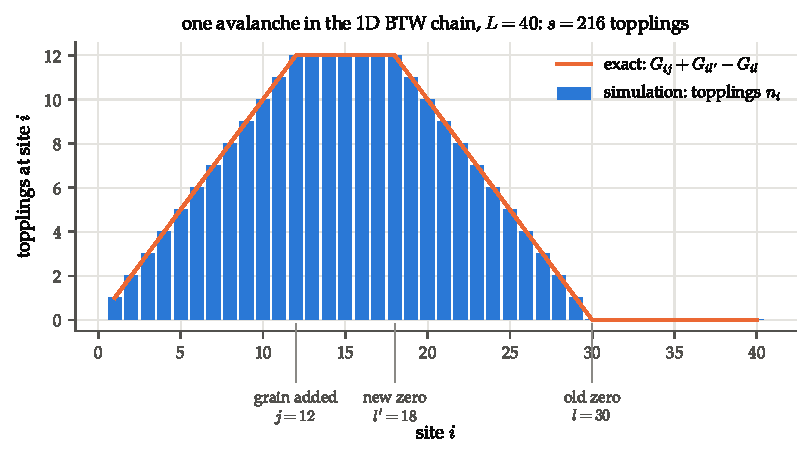
\includegraphics[width=\linewidth]{soc/btw1d_profile.pdf}
  \caption{Number of topplings at each site in one avalanche of the chain with $L=40$, $l=30$, $j=12$. Bars: simulation.
  Line: \cref{eq:n1d}. The profile is made of straight segments with kinks at the three special sites.}
  \label{fig:btw1d-profile}
\end{figure}

\subsection{The distribution of avalanche sizes}

In the stationary state each pair $(l,j)$ occurs with probability $\frac{1}{L+1}\cdot\frac1L$, so \cref{eq:s1d} determines
the whole size distribution. Its mean follows quickly: as $l$ runs over its $L+1$ values, so does $l' = (l-j)\bmod(L+1)$, so the
averages of $g(l')$ and $g(l)$ are equal and cancel, leaving
\begin{equation}
  \avg{s} = \avg{g(j)} = \frac1L\sum_{j=1}^{L}\frac{j(L+1-j)}{2} = \frac{(L+1)(L+2)}{12},
\end{equation}
in agreement with Ruelle and Sen~\cite{RuelleSen1992} and with \cref{eq:mean-s}.

To see the \emph{shape} of the distribution, let $L$ be large and measure positions in units of $L$: $x = j/L$ and
$\lambda = l/L$ are then independent and uniformly distributed between 0 and 1. Since $g(m)/L^2\to\tfrac12\,\tfrac mL(1-\tfrac mL)$,
the natural variable is the size measured in units of $L^2$,
\begin{equation}
  y = \frac{s}{L^2} = \tfrac12\left[x(1-x) + \lambda'(1-\lambda') - \lambda(1-\lambda)\right],
\end{equation}
where $\lambda' = l'/L$. By \cref{eq:zero-moves} there are two cases.
\begin{itemize}
  \item If $\lambda > x$ (the empty site is to the right of the added grain), then $\lambda' = \lambda - x$. Expanding,
    \begin{align*}
      x(1-x) + (\lambda-x)(1-\lambda+x) - \lambda(1-\lambda)
      &= x - x^2 + \lambda - \lambda^2 + 2\lambda x - x - x^2 - \lambda + \lambda^2 \\
      &= 2x(\lambda - x),
    \end{align*}
    so $y = x\,(\lambda-x)$.
  \item If $\lambda < x$, then $\lambda' = \lambda - x + 1$, and the same algebra gives $y = (1-x)(x-\lambda)$.
\end{itemize}
The second case is the mirror image of the first (replace $x\to1-x$, $\lambda\to1-\lambda$), so the two contribute equally to the
distribution. Consider the first. For a fixed $x$, the variable $u = \lambda - x$ is uniform on $[0,1-x]$, so $y = xu$ is uniform on
$[0,\,x(1-x)]$ and has density $1/x$ there. A given value $y$ can be produced only by those $x$ with $x(1-x)>y$, i.e.\ by
$x_-<x<x_+$ with $x_\pm = \tfrac12\bigl(1\pm\sqrt{1-4y}\bigr)$. Integrating over these $x$ and doubling for the mirror case,
\begin{equation}
  \boxed{\; f(y) = 2\int_{x_-}^{x_+}\frac{\dd x}{x} = 2\ln\frac{x_+}{x_-} = 2\ln\frac{1+\sqrt{1-4y}}{1-\sqrt{1-4y}},\qquad 0<y<\tfrac14. \;}
  \label{eq:fy}
\end{equation}
This is the result of Ruelle and Sen~\cite{RuelleSen1992}, here obtained in a more elementary way. The largest possible value $y=1/4$
corresponds to $x = 1/2$, $\lambda=1$: a grain added in the middle of the chain when the empty site is at the far end. Near $y=0$ the
density has a mild (logarithmic) divergence, and near $y = 1/4$ it goes to zero like a square root. Ruelle and Sen also found that the
duration, measured in units of $L$, has the density $2t$ on $0<t<1$. \Cref{fig:btw1d-dist} compares both results with simulations.

\begin{figure}[t]
  \centering
  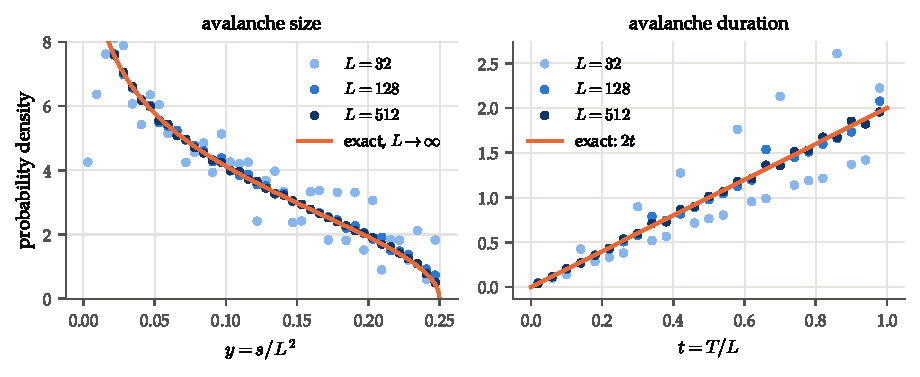
\includegraphics[width=\linewidth]{soc/btw1d_distribution.pdf}
  \caption{The one-dimensional sandpile. Left: density of the scaled avalanche size $s/L^2$ from simulations with $L = 32$, 128 and
  512 (points), and the exact large-$L$ result \cref{eq:fy} (line). Right: density of the scaled duration $T/L$ and the exact result
  $2t$. The points for $L=32$ scatter because $s$ takes only integer values. The curves for different $L$ coincide after the rescaling:
  the only scale in the problem is the system size.}
  \label{fig:btw1d-dist}
\end{figure}

\subsection{What the one-dimensional solution means}

The one-dimensional sandpile is ``critical'' only in a restricted sense. Avalanches of all sizes up to the system size occur, and there
is no length scale other than $L$. But the size distribution is \emph{not a power law}. It has the form
\begin{equation}
  P(s) = \frac{1}{L^2}\, f\!\left(\frac{s}{L^2}\right),
\end{equation}
so almost all avalanches have sizes of order $L^2$; there is no range of sizes in which $P(s)\propto s^{-\tau}$ with $\tau>1$. Compared with
\cref{eq:fss}, this corresponds to $D=2$ and an exponent $\tau=0$, and the relation \cref{eq:scaling-relation} does not apply because it
assumed $\tau>1$. The situation is similar to one-dimensional percolation (\cref{sec:perc1d}): in one dimension a single empty site can stop
or redirect an avalanche, and the critical state is too simple to produce scale-free behaviour.

This has a practical lesson for the analysis of data. Over one or two decades, a distribution like \cref{eq:fy} can look roughly straight
on a log--log plot. A straight piece of a log--log plot is therefore not proof of a power law. The reliable test is to change the system
size: a true power law extends to larger sizes with the \emph{same} slope, while a distribution like \cref{eq:fy} simply shifts as a whole.
Chapter~3 develops this into a systematic method.

% ======================================================================
\section{The two-dimensional sandpile}
\label{sec:btw2d}

On the square lattice ($k=4$, $z_c=4$, heights $0,\dots,3$) the BTW model is genuinely critical, but its exponents are not known exactly.
We present simulations with $L$ from 32 to $\socLmax$, with $\socNav$ avalanches for each $L$ after the system has reached its stationary
state. The simulation program is described in Chapter~6. We first compare with the exact results that do exist, then examine the avalanches,
and finally measure the exponents.

\subsection{Comparison with exact results}

\paragraph{Height probabilities.} For an infinitely large lattice, the probability that a site in the stationary state has height 0 was
calculated exactly by Majumdar and Dhar~\cite{MajumdarDhar1991},
\begin{equation}
  P_0 = \frac{2}{\pi^2} - \frac{4}{\pi^3} \approx 0.0736 .
\end{equation}
The probabilities of the other heights were obtained later~\cite{Priezzhev1994,JengPirouxRuelle2006}, and the mean height is exactly
$17/8 = 2.125$. (The literature uses heights $1,\dots,4$; we subtract 1.) \Cref{tab:heights} compares them with our simulation on a
$\socLmax\times\socLmax$ lattice, measured on its central part to avoid the influence of the edges. The agreement is to the third decimal.

\begin{table}[t]
\centering
\caption{Probability of each height in the stationary state of the two-dimensional BTW model.}
\label{tab:heights}
\begin{tabular}{lccccc}
\toprule
height & 0 & 1 & 2 & 3 & mean \\
\midrule
exact, infinite lattice & 0.0736 & 0.1739 & 0.3063 & 0.4462 & 2.1250 \\
simulation, $L=\socLmax$ & \socHeightSim{0} & \socHeightSim{1} & \socHeightSim{2} & \socHeightSim{3} & \socMeanHeightSim \\
\bottomrule
\end{tabular}
\end{table}

\paragraph{Mean avalanche size.} \Cref{eq:mean-s} can be evaluated for each $L$ by solving one linear system. For $L=\socLmax$ it gives
$\avg{s} = \socMeanExact$, and the simulation gives $\socMeanSim$. \Cref{fig:btw2d-moments} (left) shows the comparison for all $L$:
$\avg{s}$ grows as $L^2$, as \cref{eq:mean-L2} requires, and the simulation agrees with the exact value at every size.

\subsection{The avalanches}

\Cref{fig:btw2d-snapshot} shows one large avalanche. The region that toppled is compact, and the number of topplings per site increases in
nested, roughly concentric layers towards the site where the grain was added. Each layer corresponds to a ``wave'': the starting site
topples, a wave of topplings spreads out, and when it has died the starting site may be unstable again and start the next wave. Priezzhev,
Ktitarev and Ivashkevich~\cite{Priezzhev1996} showed that single waves are much simpler objects than whole avalanches (the exponent of their
size distribution, $11/8$, can be calculated exactly), and that the difficulty of the BTW model lies in how waves stack up into avalanches.

\begin{figure}[t]
  \centering
  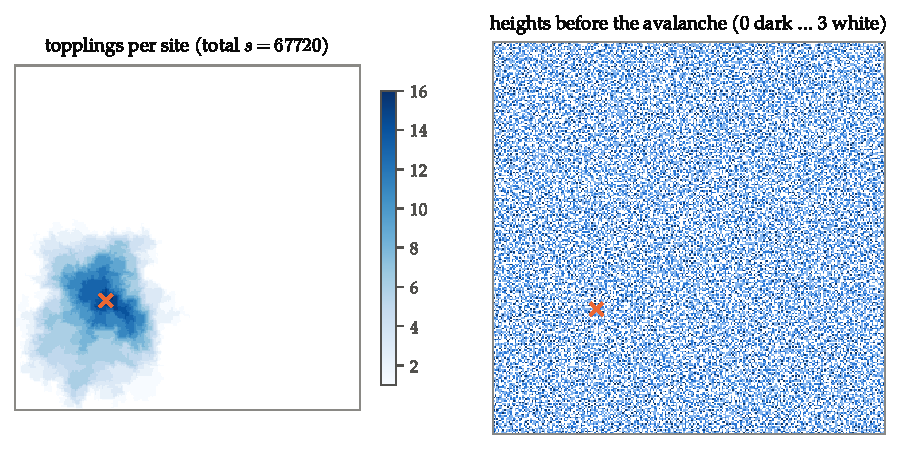
\includegraphics[width=\linewidth]{soc/btw2d_snapshot.pdf}
  \caption{One large avalanche on a $256\times256$ lattice; the grain was added at the site marked $\times$. Left: number of topplings at each
  site. Right: the heights just before the grain was added.}
  \label{fig:btw2d-snapshot}
\end{figure}

\Cref{fig:btw2d-dist} shows the distributions of size, area and duration. Unlike in one dimension, each distribution has a straight
section on the log--log plot whose slope \emph{does not change} with $L$; increasing $L$ only extends the straight section to larger
values, as in \cref{eq:fss}. This is the signature of genuine critical behaviour. A guide line with slope $-1.2$ is drawn for the size
distribution, but its local slope drifts slowly, and fitting a straight line by eye is not a reliable way to obtain $\tau$.

\begin{figure}[t]
  \centering
  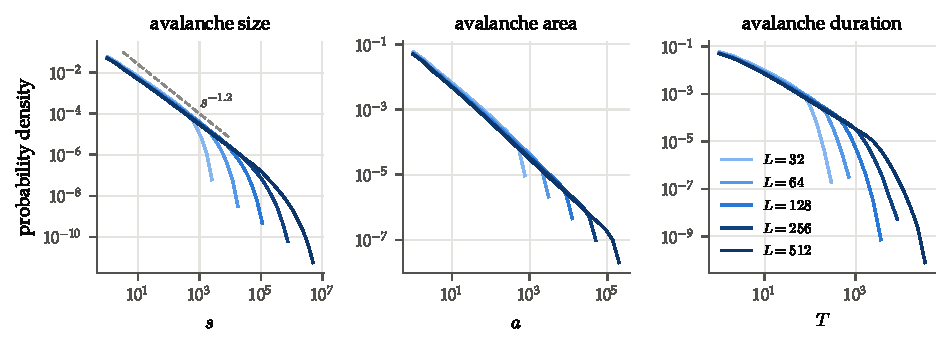
\includegraphics[width=\linewidth]{soc/btw2d_distributions.pdf}
  \caption{Two-dimensional BTW sandpile: probability densities of avalanche size, area and duration for $L = 32$, 64, 128, 256 and 512
  (light to dark). Logarithmically spaced bins are used so that each decade has the same number of points.}
  \label{fig:btw2d-dist}
\end{figure}

\subsection{Measuring the exponents with moments}

A more reliable method uses the moments of the distribution instead of its shape. Assume the form \cref{eq:fss},
$P(s) = s^{-\tau}\mathcal G(s/s_c)$ with $s_c = c\,L^{D}$. The $q$-th moment is
\begin{equation}
  \avg{s^q} = \int s^{q}\, s^{-\tau}\,\mathcal G\!\left(\frac{s}{s_c}\right)\dd s .
\end{equation}
Substitute $s = s_c u$, $\dd s = s_c\,\dd u$:
\begin{equation}
  \avg{s^q} = s_c^{\,q+1-\tau}\int u^{q-\tau}\,\mathcal G(u)\,\dd u \;\propto\; L^{D(q+1-\tau)} .
\end{equation}
The remaining integral is a number independent of $L$, provided $q>\tau-1$ so that it converges at small $u$ (for smaller $q$ the small
avalanches dominate and the moment does not grow with $L$). Defining the \emph{moment exponent} $\sigma(q)$ by $\avg{s^q}\propto L^{\sigma(q)}$,
\begin{equation}
  \sigma(q) = D\,(q+1-\tau) .
  \label{eq:moments}
\end{equation}
So $\sigma(q)$ is a straight line in $q$ with slope $D$. Each $\sigma(q)$ is measured as the slope of $\log\avg{s^q}$ against $\log L$. This uses
all the data, requires no binning and no choice of a fitting window in $s$. As a check, $\sigma(1) = D(2-\tau)$ must equal 2 by
\cref{eq:scaling-relation}.

\Cref{fig:btw2d-moments} (right) shows the measured $\sigma(q)$. The value at $q=1$ is 2, as it must be, and the slope for $q\ge2$ gives
$D\approx\socDest$. With \cref{eq:scaling-relation}, $\tau = 2-2/D \approx \socTauRel$. Large-scale simulations by Lübeck and
Usadel~\cite{LubeckUsadel1997} give $\tau\approx1.29$ and $D\approx2.73$. Our $\tau$ agrees; our $D$ is about 3\% larger, which is not
surprising for system sizes up to $\socLmax$ and a slope estimated from three sizes. Part of the difference, however, is a real property of
the model: on close inspection $\sigma(q)$ is not exactly a straight line. Tebaldi, De Menech and Stella~\cite{Tebaldi1999} showed that the BTW
model does not follow the simple form \cref{eq:fss} exactly: small and large avalanches scale with slightly different exponents, a property
called \emph{multifractality}. For the BTW model, therefore, ``the'' value of $\tau$ depends somewhat on how it is measured. Other sandpile
models, such as the stochastic Manna model, follow \cref{eq:fss} much more cleanly.

\begin{figure}[t]
  \centering
  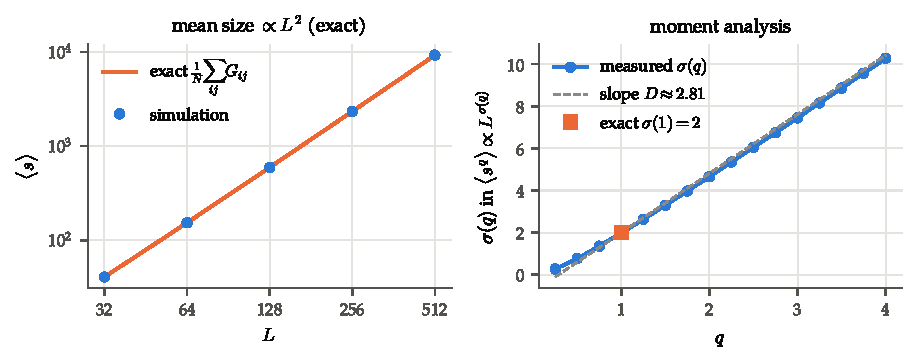
\includegraphics[width=\linewidth]{soc/btw2d_moments.pdf}
  \caption{Two-dimensional BTW sandpile. Left: mean avalanche size against $L$; the line is the exact \cref{eq:mean-s}, the points are
  simulations. Right: moment exponents $\sigma(q)$, obtained from the three largest system sizes; the dashed line has the slope $D$ fitted for
  $q\ge2$, and the square marks the exact value $\sigma(1)=2$.}
  \label{fig:btw2d-moments}
\end{figure}

% ======================================================================
\section{Summary and implications for the Burridge--Knopoff model}
\label{sec:soc-implications}

The main points of this chapter are:
\begin{itemize}
  \item A power law $P(x)\propto x^{-\tau}$ is the only distribution without a characteristic scale. In ordinary statistical physics it appears
    only at a critical point, which must be reached by tuning a control parameter.
  \item Self-organized criticality is the proposal that slow driving, a local threshold, fast local relaxation and dissipation drive a system to
    its critical point without tuning. The feedback argument of \cref{sec:soc} shows why, and also that it requires the limits of vanishing
    driving rate and vanishing bulk dissipation.
  \item The BTW sandpile is Abelian. This gives exact results: all recurrent configurations are equally likely, the mean number of topplings is
    the Green function, $\avg{s}\propto L^2$, and $D(2-\tau)=2$.
  \item In one dimension the BTW model is solved exactly: an added grain moves the single empty site by $j$ places, the avalanche size is
    $s = g(j) + g(l') - g(l)$, and the size distribution is a function of $s/L^2$ that is \emph{not} a power law.
  \item In two dimensions the BTW model is critical, with $\tau\approx1.2$--$1.3$ and $D\approx2.7$--$2.8$, and small deviations from simple
    scaling.
\end{itemize}

Three of these points shape the rest of this thesis.

\emph{One dimension.} The Burridge--Knopoff model studied here is one-dimensional, and the simplest one-dimensional sandpile is not
critical. Whatever broad distribution of event sizes the Burridge--Knopoff model produces must therefore come from features that the
one-dimensional BTW model does not have: continuous rather than integer variables, deterministic rather than random driving, or the inertia of
the blocks.

\emph{Bulk dissipation.} In the sandpile, grains are lost only at the edges, and this is what makes $\avg{s}\propto L^2$ and the cutoff grow with
the system size. In the Burridge--Knopoff model every block is attached to the moving plate by a pulling spring. When a block slips, part of the
force it releases goes into its own pulling spring rather than to its neighbours, so stress is lost \emph{inside} the system. In the language of
the random-walk picture of \cref{sec:mean}, a grain that is lost with probability $\epsilon$ at each step travels on average only a distance of
order $\epsilon^{-1/2}$ before it disappears. Such bulk dissipation introduces a length scale that does not depend on $L$, and avalanches larger
than this scale are suppressed. For the Burridge--Knopoff model this length turns out to be set by the ratio of the two spring constants,
$\ell = \sqrt{k_c/k_p}$, as will be shown in Chapters~4 and~5.

\emph{Uniform driving.} In the sandpile, grains are added at random sites; in the Burridge--Knopoff model the plate loads all blocks
simultaneously and deterministically. The model that combines continuous variables, uniform driving and bulk dissipation is the
Olami--Feder--Christensen model~\cite{OFC1992}, which will be the starting point of the mapping in Chapter~5.
